\clearpage{}
\section{Define the stages of a software lifecycle. Describe and compare the
waterfall model, the V model, the spiral model and the agile model of
software development. Discuss the addition of prototyping.}

\subsection{Stages of a software lifecycle}

The \textbf{software life cycle}, also called \textbf{software process}, has the following stages:

\begin{enumerate}
    \item \textbf{Requirements analysis and definition}\\
    Expression of the desired behavior (\textit{what} behavior is needed, but \textit{not how} it is actually realized).
    \item \textbf{System (architecture) design}\\
     Description of \textit{how} to implement the customer's requirements (decomposition in software units, specifying interfaces, protocols and data,\ldots)
    \item \textbf{Program (detailed) design}\\
     Translation of the architecture design into a program (how each software unit will be built). The basis for writing code.
    \item \textbf{Program writing}\\
     Proper implementation of the solution.
    \item \textbf{Unit testing}\\
     Check that the code properly implements the design and involves software developers to achieve it.
     These kind of test are to test small parts of the software.
    \item \textbf{Integration testing}\\
     Another part of \textit{program testing} along with unit testing. They are used to detect bugs
     errors that cannot be detected with unit testing.
    \item \textbf{System testing}\\
    Check that the system does what the customer wants and involves the whole development team to achieve it.
    \item \textbf{System delivery}\\
     More than just handing the product over but helping the users to understand and make good use of the whole system.
    \item \textbf{Maintenance}
    System maintenance involve all the operation that occurs after the delivery of the systems such as 
    improving performance or correcting faults.
\end{enumerate}

\subsection{The waterfall model} The waterfall model was one of the first
models proposed, it is a simple basis for defining more complex models. Stages are depicted as cascading from one to another (i.e. one development stage should be completed before the next begins).\\

It can be used for well understood problems that have stable requirements. For example if you are at the version 36 of your accounting software with stable customer needs, this process works pretty well.\\

Thanks to its very high-level view, the Waterfall model is simple and easy to understand.
However, it cannot handle changes (frozen requirements, manufacturing process rather than creative, no iterative activities) and there is a long wait before a final product.

\begin{figure}[!ht]
    \centering
    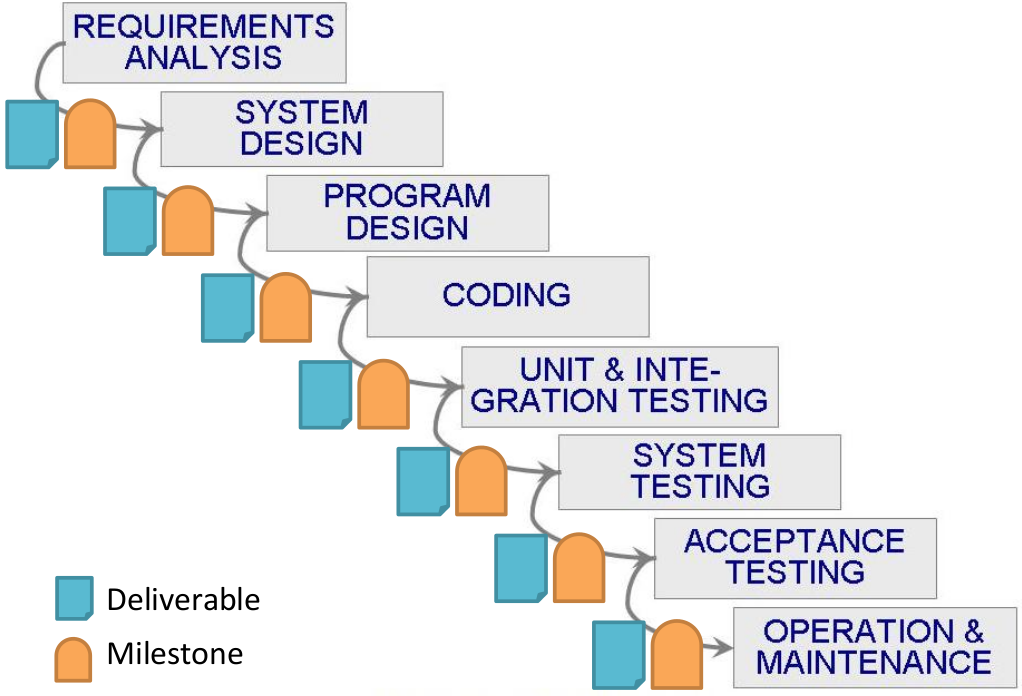
\includegraphics[width=0.6\linewidth]{waterfall_plus.png}
    \caption{Waterfall model lifecycle}
\end{figure}
\FloatBarrier{}

\subsection{The V model}

The V model is a variation of the waterfall model that separates it in two phases: \textbf{development} (design) and \textbf{testing} (V\&V\footnote{Verification and
validation}).\\

It shows how the testing activities are related to the analysis and design. Indeed, if problems are found during the testing activities, it is possible to loop back to the left side of the V and re-thinks a part of the analysis and design with a better understanding of the problem so V model provide a bit more flexibility than the 
waterfall model.

\begin{figure}[!ht]
    \centering
    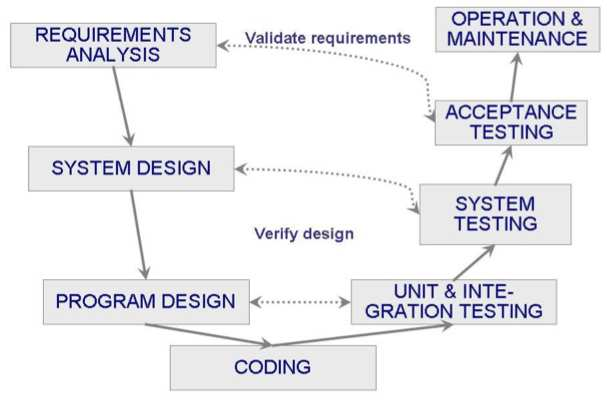
\includegraphics[width=0.6\linewidth]{v_model_2.png}
    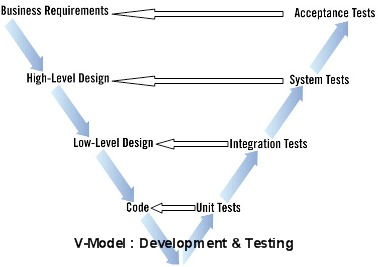
\includegraphics[width=0.6\linewidth]{v_model.png}
    \caption{V model lifecycle}
\end{figure}
\FloatBarrier{}

\subsection{The spiral model}
This model combines both the development activities with the risk management to minimize and
control the risk. It is a sort of iterative development (full system at the very
beginning and then changes functionality of each subsystem with each new
release). \newline

Four basic activites that must occur in each cycle of the spiral model:

\begin{enumerate}
    \item Consider the win conditions of all success-critical stakeholders.
    \item Identify and evaluate alternative approaches for satisfying the win
    conditions.
    \item Identify and resolve risks that stem from the selected approach(es)
    (e.g.\ you can try resolve it, by making a prototype which valid the
    approach).
    \item Obtain approval from all success-critical stakeholders, plus
    commitment to pursue the next cycle.
\end{enumerate}

\begin{figure}[!ht]
    \centering
    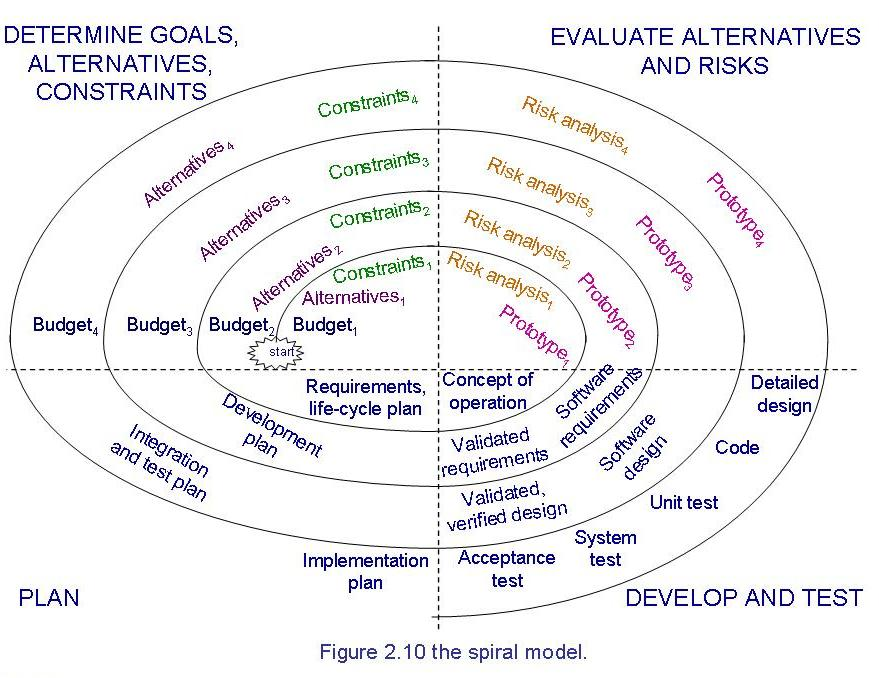
\includegraphics[width=0.8\linewidth]{spiral_model.png}
    \caption{Spiral model lifecycle}
\end{figure}
\FloatBarrier{}

\subsection{Agile model}
The classical software development process models are rigorous process for
software conception, documentation, development and testing. The alternative is the agile method that is a flexible process that can adapt to changing requirements. The overall goal of agile development is to satisfy the customer by \enquote{early and continuous delivery of valuable software}.

\paragraph{Agile Manifesto :\\}

\begin{itemize}
    \item Value individuals and interactions over processes and tools
    \item Prefer to invest time in producing working software rather than in producing comprehensive documentation
    \item Focus on customer collaboration rather than contract negotiation
    \item Concentrate on responding to change rather than on creating a plan and then following it
\end{itemize}


\paragraph{Examples of agile processes :\\}

\begin{itemize}
    \item Extreme programming (XP)
    \item Crystal
    \item Scrum
\end{itemize}

\subsection{Addition of prototyping}

Prototyping means building a small version of a system (usually with limited
functionality) that can be used to:

\begin{itemize}
    \item Demonstrate the feasibility of a design or approach
    \item Help the user (or customer) to identify key requirements of a system
\end{itemize}


Often, the prototyping is iterative: We build a prototype, evaluate it (with
user and customer feedback), consider how changes might improve the product or
design, and then build another prototype. The iteration ends when our customers
and we think we have a satisfactory solution to the problem at hand.

\paragraph{Imagine, in detail, a new product is... hard.}
\paragraph{Criticize, in detail, an existing product is... easier.\\
 $\rightarrow$ That's prototyping.}

\paragraph{}

There are two main approaches to prototyping :

\begin{itemize}
    \item \textbf{Throwaway :} software developed to learn more about the
    problem/proposed solution. “Quick and dirty” software that will be thrown
    away (not part of the delivered software).
    \item \textbf{Evolutionary :} software developed not only to help us answer questions
    but also to be incorporated into the final product.
\end{itemize}
